\documentclass[11pt]{article}

\usepackage[letterpaper,margin=0.75in]{geometry}
\usepackage{booktabs}
\usepackage{graphicx}
\usepackage{listings}

\setlength{\parindent}{1.4em}

\begin{document}

\lstset{
  language=Python,
  basicstyle=\small,          % print whole listing small
  keywordstyle=\bfseries,
  identifierstyle=,           % nothing happens
  commentstyle=,              % white comments
  stringstyle=\ttfamily,      % typewriter type for strings
  showstringspaces=false,     % no special string spaces
  numbers=left,
  numberstyle=\tiny,
  numbersep=5pt,
  frame=tb,
}

\title{Reliable Transport}

\author{Jonathan George}

\date{}

\maketitle

\section{Description}
In this lab, we have added conguestion control to our bene simulator. We used the simulator data to examine the correctness of our implementation in several situations.

\section{Conguestion Control}
Conguestion control for TCP consists of several main pieces. First, at the start of any connection we begin in slow start with a conguestion window of size 1. This window increases by the maximum segment size each time we recieve an new ack. When the conguestion window grows larger than the threshold, then we no longer increase for every ack, but instead after each full window we send. As the window size increases, then the threshold also increases to match it. This is called Additive Increase. The code below from tcp.py illustrated these two principles.

\begin{lstlisting}
def adjustWindow(self):
    #adjust window size
    if self.window >= self.threshold: #
        if self.ackCount >= float(self.window)/self.mss:
            self.window += self.mss
            self.threshold += self.mss
            self.ackCount = 0
        else:
            self.ackCount += 1
    else:
        self.window += self.mss
\end{lstlisting}

In addition to Additive Increase Multiplicative Decrease, TCP also includes Fast Retransmit. Whenever three duplicate acks are detected (meaning the fourth time we recieve the same ACK), then we trigger a loss event. Loss events restart the conguestion window back to one maximum segment size and it begins again in slow start. The threshold will also be reduced into half to a minimum of one maximum segment size. Then we trigger a retransmit event as if we had a timeout event. 

\begin{lstlisting}
def lossEvent(self):
    self.threshold = max(self.window/2,self.mss)
    self.window = self.mss
\end{lstlisting}

\section{Tests Description}
In order to prove our implementation of TCP conguestion control works, we have creating a graphing script to create graphs similar to the Sally Floyd paper we discussed in class.[1] These graphs shows when packets are sent, lost and acknowledged. Below we have analyzed, slow start, additive increase, packet loss and burst packet loss.

\section{Slow Start Graph}

In this test we transfered a small file such that the entire transmission occurs during slow start, with no loss. The window size should grew larger 32 packets all during slow start.

\centerline{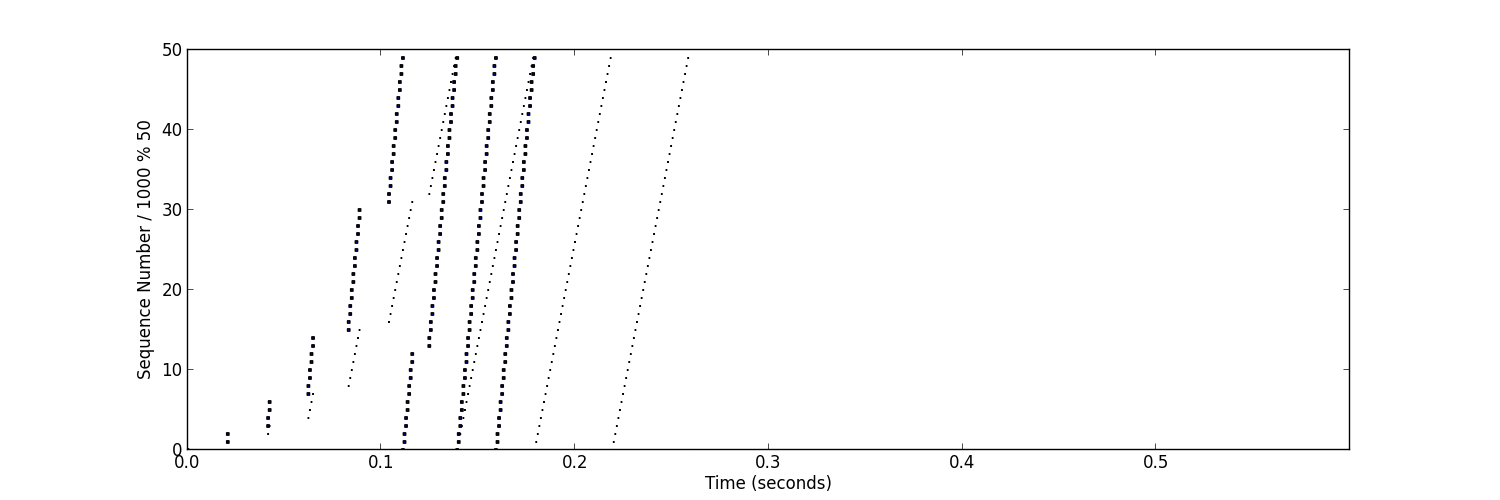
\includegraphics[width=22cm]{slow_start.png}}

\section{Additive Increase Graph}

We repeated the above experiment, but with a slow start threshold of 16000 bytes (16 packets). This shows that our implementation switches to additive increase when the window size becomes larger than the threshold.

\centerline{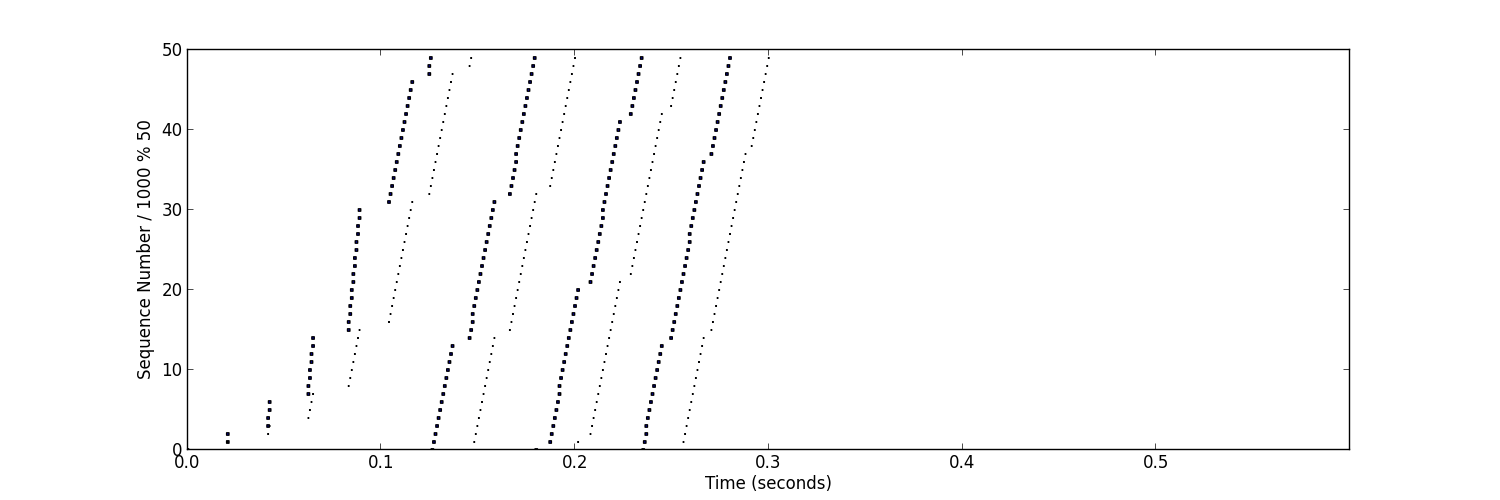
\includegraphics[width=22cm]{additive_increase.png}}

\section{AIMD Graph}

In this experiement, we purposefully dropped the first packet when the window size had grown to 32. We can see from the graph that the window was reduced back to 1 MSS and the threshold also was reduced in half. 

\centerline{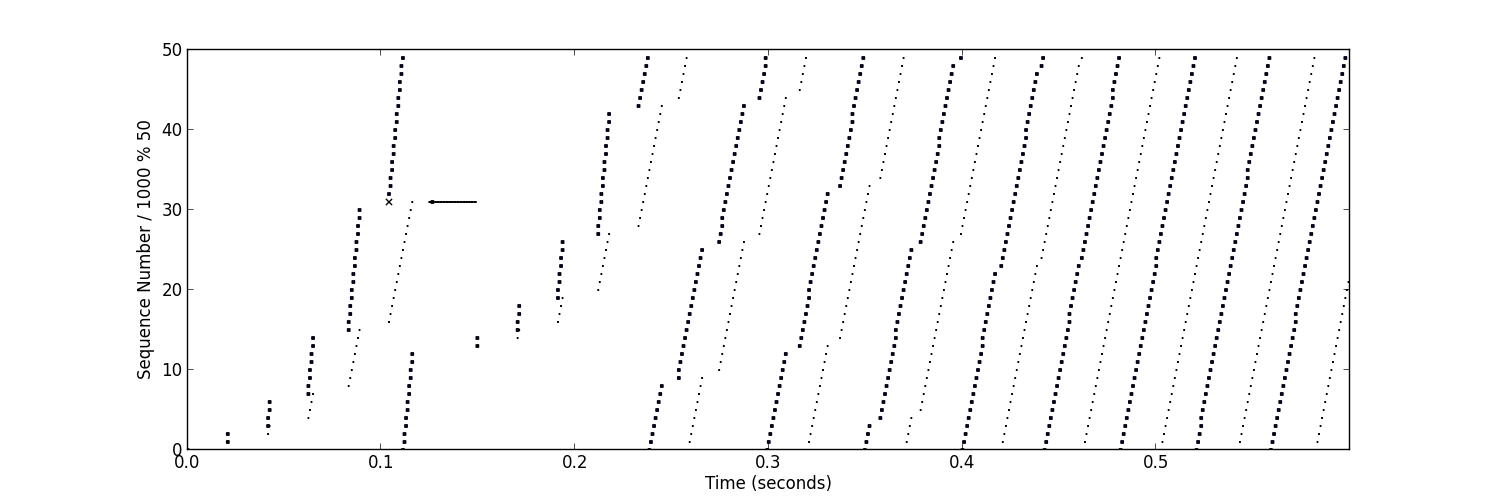
\includegraphics[width=22cm]{AIMD.png}}

\section{Burst Loss Graph}

Finally, we have experiemented with the situation where multiple packets are lost in a quick burst. In this situation, we can see that TCP reacts appropriately and recovers quickly without issue.

\centerline{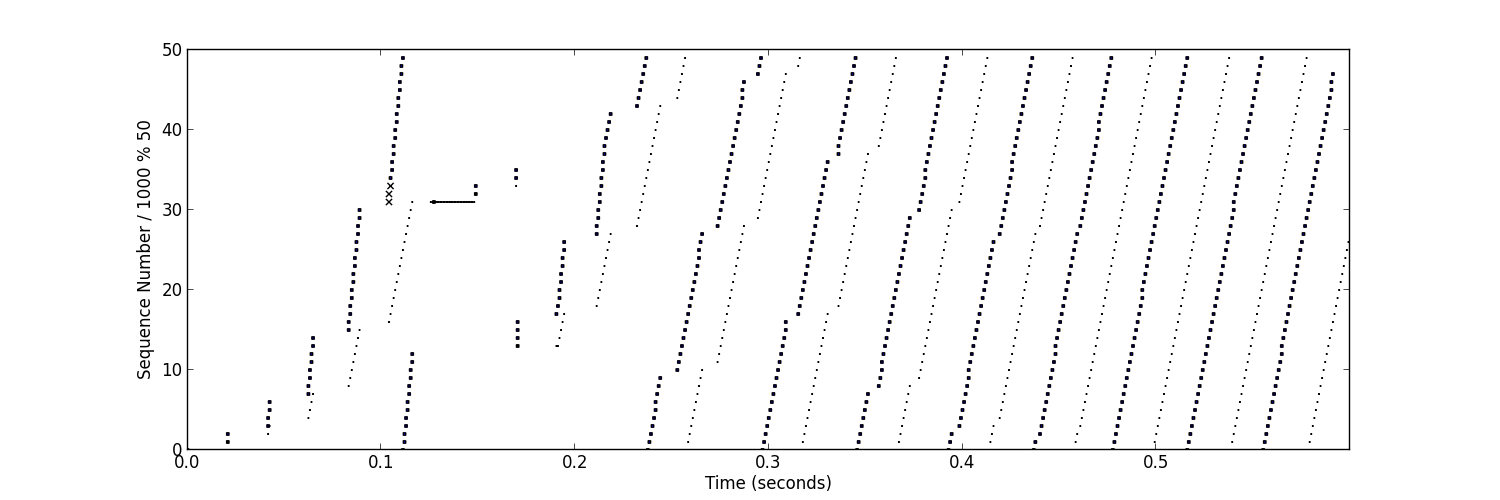
\includegraphics[width=22cm]{burst_loss.png}}

\section{TCP Reno}
We also implemented TCP reno. TCP reno is identical to TCP Tahoe, but instead of returning to slow start after a loss event it sets the window size to half of the previous window size. The first graph below shows that it does improve a single loss event situation. However, in the second graph we can see that multiple losses cause Reno to have multiple loss events. This causes the threshold size to drop rapidly.

\centerline{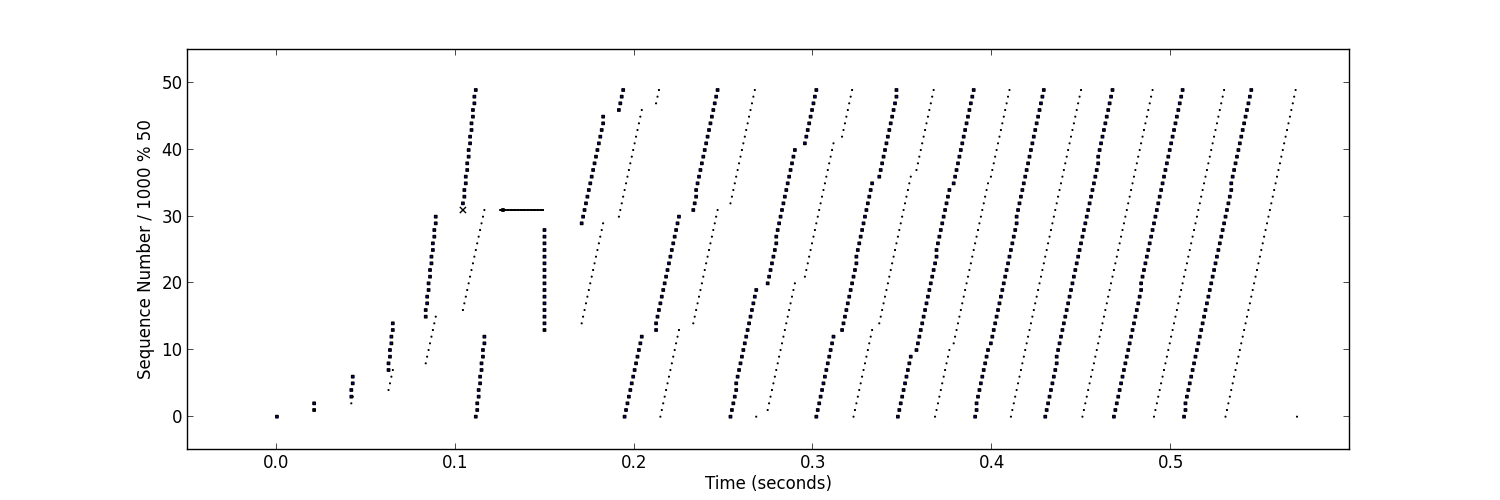
\includegraphics[width=22cm]{AIMD_reno.png}}

\centerline{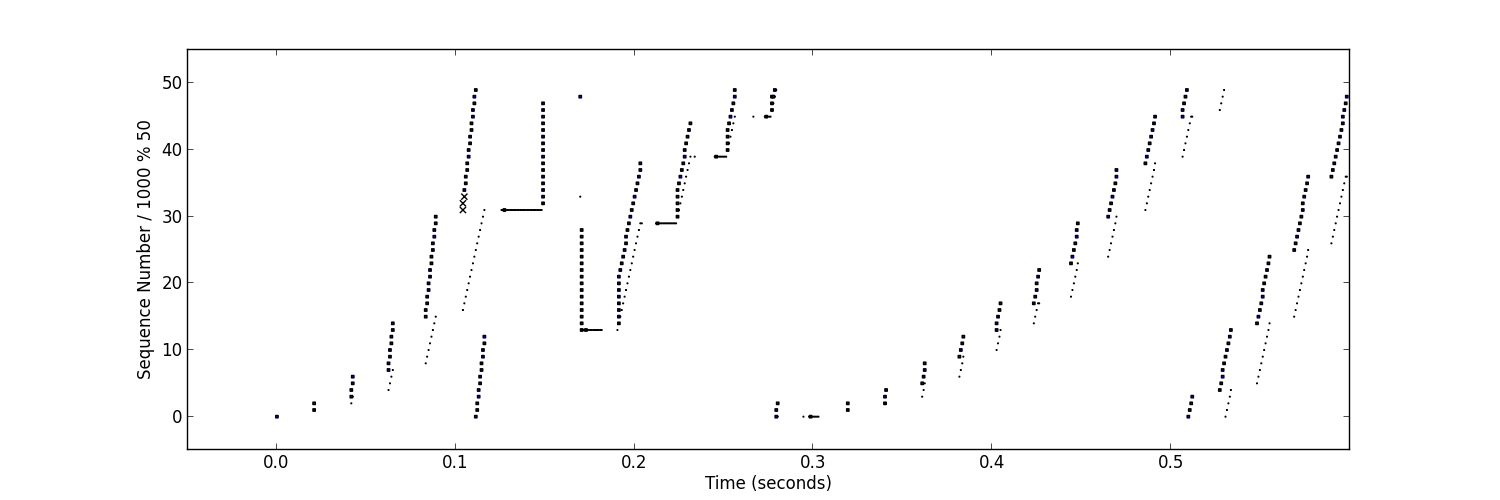
\includegraphics[width=22cm]{burst_loss_reno.png}}

\section{Works Cited}

[1] Kevin Fall and Sally Floyd, Simulation-based Comparisons of Tahoe, Reno, and SACK TCP, ACM Computer Communications Review, Volume 26, Number 3, July, 1996

\end{document}
